\documentclass[11pt]{article}
%\usepackage{fullpage}
\usepackage[top=2cm, bottom=1.5cm, left=1.5cm, right=1.5cm]{geometry}
\usepackage{amsmath,amsthm,amsfonts,amssymb,amscd}
\usepackage{xcolor}
\usepackage{graphicx}
\usepackage[utf8]{inputenc}
\usepackage[english]{babel}
\usepackage{fancyhdr}
\usepackage{wrapfig}

\pagestyle{fancy}
\fancyhf{}
\fancyhead[LO]{Mechanics \& Relativity F3210}
\fancyhead[RO]{Workshop 9: Fluids}
%\fancyfoot[CE,CO]{\leftmark}
%\fancyfoot[LE,RO]{\thepage}

%answers
\usepackage{etoolbox}
\providetoggle{answers}
\settoggle{answers}{false}

\newcommand\vect[1]{\underline{\mathbf{#1}}}
\newcommand\unitvect[1]{\hat{\boldsymbol{#1}}}

\begin{document}

\noindent
\textbf{\textcolor{red}{Please upload your solution to Problem 3 to canvas for marking after the workshop.}}\\

\section*{Problem 1}

Anyone who scuba dives is advised not to fly within the next 24 h because the air mixture for diving can introduce nitrogen to the bloodstream. Without allowing the nitrogen to come out of solution slowly, any sudden air-pressure reduction (such as during airplane ascent) can result in the nitrogen forming bubbles in the blood, creating the bends, which can be painful and even fatal. Military special operation forces are especially at risk. What is the change in pressure on such a special-op soldier who must scuba dive at a depth of 20 m in seawater one day and parachute at an altitude of 7.6 km the next day? Assume that the average air density within the altitude range is 0.87 kgm$^{-3}$

\noindent

\section*{Problem 2}

A boat floating in fresh water displaces water weighing 35.6 kN.\\
 (a) What is the weight of the water this boat displaces when floating in salt water of density $1.10 \times 10^3$ kgm$^{-3}$? \\
 (b) What is the difference between the volume of fresh water displaced and the volume of salt water displaced?


\section*{\textcolor{red}{Problem 3}}
\fbox{\begin{minipage}{\textwidth}
Models of torpedoes are sometimes tested in a horizontal pipe of flowing water, much as a wind tunnel is used to test model airplanes. Consider a circular pipe of internal diameter 25.0 cm and a torpedo model aligned along the long axis of the pipe. The model has a 5.00 cm diameter and is to be tested with water flowing past it at 2.50 ms$^{-1}$.\\
 (a) With what speed must the water flow in the part of the pipe that is unconstricted by the model? \\
 (b) What will the pressure difference be between the constricted and unconstricted parts of the pipe?
\end{minipage}}



\section*{Problem 4}

Two streams merge to form a river. One stream has a width of 8.2 m, depth of 3.4 m, and current speed of 2.3 ms$^{-1}$. The other stream is 6.8 m wide and 3.2 m deep, and flows at 2.6 ms$^{-1}$. If the river has width 10.5 m and speed 2.9 ms$^{-1}$, what is its depth?

%\vspace{0.5cm}
\section*{Want more practice?}
\small
Further problems on Fluids: Chapter 14 \\



\begin{figure}[h]
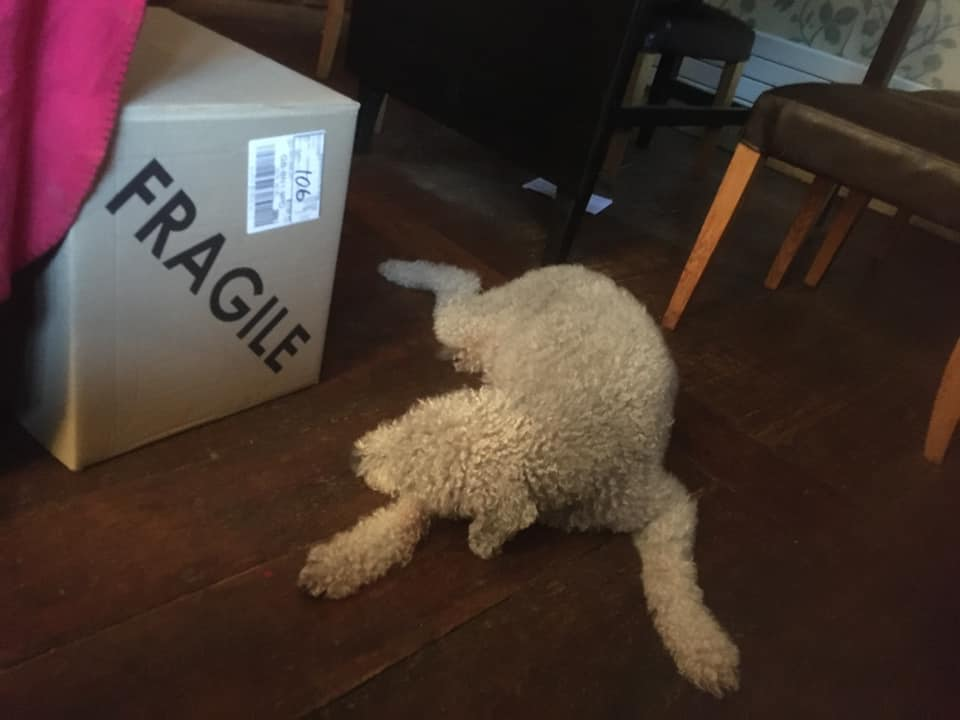
\includegraphics[scale=0.15]{sploot.jpg}
\end{figure}


\end{document}
 




 


